\begin{exercise}
      {ID-65244850a6f18971e9d4b9a2867d7c139ed63dab}
      {Grad 4}
  \ifproblem\problem\par
    % <PROBLEM>
    Bestimmen Sie -- falls existent -- die Gleichung
    einer ganzrationalen Funktion vierten Grades.
    deren zur $y$-Achse symmetrischer Graph durch
    $Q\left(1\;\middle|\;2\right)$ geht und bei
    $x=2$ die $x$-Achse berührt.
    % </PROBLEM>
  \fi
  \ifoutline\outline\par
    % <OUTLINE>
    Folgende Informationen sind in der
    Aufgabenstellung gegeben:
    \begin{enumerate}[a)]
      \item $f$ ist eine ganzrationale Funktion
            vierten Grades
      \item $f$ ist symmetrisch zur $y$-Achse
      \item $Q\left(1\;\middle|\;2\right)$ liegt
            auf dem Graphen von $f$
      \item $f$ \emph{berührt} die $x$-Achse bei
            $x=2$
    \end{enumerate}
    % </OUTLINE>
  \fi
  \ifoutcome\outcome\par
    % <OUTCOME>
    Folgende Informationen sind in der
    Aufgabenstellung gegeben:
    \begin{enumerate}[a)]
      \item $f$ ist eine ganzrationale Funktion
            vierten Grades:
            \begin{equation*}
              f(x)=ax^4+bx^3+cx^2+dx+e
            \end{equation*}
      \item $f$ ist symmetrisch zur $y$-Achse,
            d.\,h. es gibt keine ungeraden
            Exponenten im Funktionsterm:
            \begin{equation*}
              b=0
              \quad\text{und}\quad
              d=0
            \end{equation*}
      \item $Q\left(1\;\middle|\;2\right)$ liegt
            auf dem Graphen von $f$:
            \begin{equation*}
              f(1)=2
            \end{equation*}
      \item $f$ \emph{berührt} die $x$-Achse bei
            $x=2$:
            \begin{equation*}
              f(2)=0
              \quad\text{und}\quad
              f'(2)=0
            \end{equation*}
    \end{enumerate}
    Die gesuchste Funktion und deren erste Ableitung
    haben also folgende vorläufige Form:
    \begin{equation*}
      f(x)=ax^4+cx^2+e
      \quad\text{und}\quad
      f'(x)=4ax^3+2cx
    \end{equation*}
    Die noch unbekannten Koeffizienten $a$, $c$ und
    $e$ ergeben sich dann aus folgendem
    Gleichungssystem:
    \begin{equation*}
      \setlength{\arraycolsep}{0.1em}%
      \begin{array}{r|lcr}
          \text{I}\;\; & \; f(1)  & = & 2 \\
         \text{II}\;\; & \; f(2)  & = & 0 \\
        \text{III}\;\; & \; f'(2) & = & 0
      \end{array}
      \quad\Rightarrow\quad
      \begin{array}{r|rcrcrcr}
          \text{I}\;\; & \;  a\cdot1^4 & + &  c\cdot1^2 & + & e & = & 2 \\
         \text{II}\;\; & \;  a\cdot2^4 & + &  c\cdot2^2 & + & e & = & 0 \\
        \text{III}\;\; & \; 4a\cdot2^3 & + & 2c\cdot2   &   &   & = & 0
      \end{array}
    \end{equation*}
    \par Als Lösung erhält man:\\
    \begin{minipage}[t]{0.49\linewidth}
      \vspace*{-\abovedisplayskip}
      \begin{alignat*}{1}
        % <STEP>
        &\setlength{\arraycolsep}{0.1em}%
        \begin{array}{r|rrrrrrrrrl}
          \text{I}{\,} & {\,} &  \num{1}a & + & \num{1}c & + & \num{1}e & = & \num{2} & {\quad} &            \\
         \text{II}{\,} & {\,} & \num{16}a & + & \num{4}c & + & \num{1}e & = & \num{0} & {\quad} & |-\text{I} \\
        \text{III}{\,} & {\,} & \num{32}a & + & \num{4}c & + & \num{0}e & = & \num{0} & {\quad} &
        \end{array}
        % </STEP>
        % <STEP>
        \\[1ex]&\setlength{\arraycolsep}{0.1em}%
        \begin{array}{r|rrrrrrrrrl}
          \text{I}{\,} & {\,} &  \num{1}a & + & \num{1}c & + & \num{1}e & = &  \num{2} & {\quad} &                                     \\
         \text{II}{\,} & {\,} & \num{15}a & + & \num{3}c & + & \num{0}e & = & -\num{2} & {\quad} &                                     \\
        \text{III}{\,} & {\,} & \num{32}a & + & \num{4}c & + & \num{0}e & = &  \num{0} & {\quad} & |\cdot\num{3}-\num{4}\cdot\text{II}
        \end{array}
        % </STEP>
        % <STEP>
        \\[1ex]&\setlength{\arraycolsep}{0.1em}%
        \begin{array}{r|rrrrrrrrrl}
          \text{I}{\,} & {\,} &  \num{1}a & + & \num{1}c & + & \num{1}e & = &  \num{2} & {\quad} &           \\
         \text{II}{\,} & {\,} & \num{15}a & + & \num{3}c & + & \num{0}e & = & -\num{2} & {\quad} &           \\
        \text{III}{\,} & {\,} & \num{36}a & + & \num{0}c & + & \num{0}e & = &  \num{8} & {\quad} & |:\num{4}
        \end{array}
        % </STEP>
      \end{alignat*}
    \end{minipage}%
    \hfill
    \begin{minipage}[t]{0.49\linewidth}
      \vspace*{-\abovedisplayskip}
      \begin{alignat*}{1}
        % <STEP>
        &\setlength{\arraycolsep}{0.1em}%
        \begin{array}{r|rrrrrrrrrl}
          \text{I}{\,} & {\,} &  \num{1}a & + & \num{1}c & + & \num{1}e & = &  \num{2} & {\quad} & |\cdot\num{9}-\text{III}             \\
         \text{II}{\,} & {\,} & \num{15}a & + & \num{3}c & + & \num{0}e & = & -\num{2} & {\quad} & |\cdot\num{3}-\num{5}\cdot\text{III} \\
        \text{III}{\,} & {\,} &  \num{9}a & + & \num{0}c & + & \num{0}e & = &  \num{2} & {\quad} &
        \end{array}
        % </STEP>
        % <STEP>
        \\[1ex]&\setlength{\arraycolsep}{0.1em}%
        \begin{array}{r|rrrrrrrrrl}
          \text{I}{\,} & {\,} & \num{0}a & + & \num{9}c & + & \num{9}e & = &  \num{16} & {\quad} & |-\text{II} \\
         \text{II}{\,} & {\,} & \num{0}a & + & \num{9}c & + & \num{0}e & = & -\num{16} & {\quad} &             \\
        \text{III}{\,} & {\,} & \num{9}a & + & \num{0}c & + & \num{0}e & = &   \num{2} & {\quad} &
        \end{array}
        % </STEP>
        % <STEP>
        \\[1ex]&\setlength{\arraycolsep}{0.1em}%
        \begin{array}{r|rrrrrrrrrl}
          \text{I}{\,} & {\,} & \num{0}a & + & \num{0}c & + & \num{9}e & = &  \num{32} & {\quad} &   \\
         \text{II}{\,} & {\,} & \num{0}a & + & \num{9}c & + & \num{0}e & = & -\num{16} & {\quad} &   \\
        \text{III}{\,} & {\,} & \num{9}a & + & \num{0}c & + & \num{0}e & = &   \num{2} & {\quad} &
        \end{array}
        % </STEP>
      \end{alignat*}
    \end{minipage}\par
    Der gesuchte Funktionsterm lautet also:
    \begin{equation*}
      %<OCTAVE>
      f(x)=\frac{\num{2}}{\num{9}}x^{4}-\frac{\num{16}}{\num{9}}x^{2}+\frac{\num{32}}{\num{9}}
      %</OCTAVE>
      %f = [2/9 0 -16/9 0 32/9];
      %printf("f(x)=%s\n", mypolystr(f, "x", [0,0,0,0,1]));
    \end{equation*}
    \begin{center}
      %<OCTAVE>
      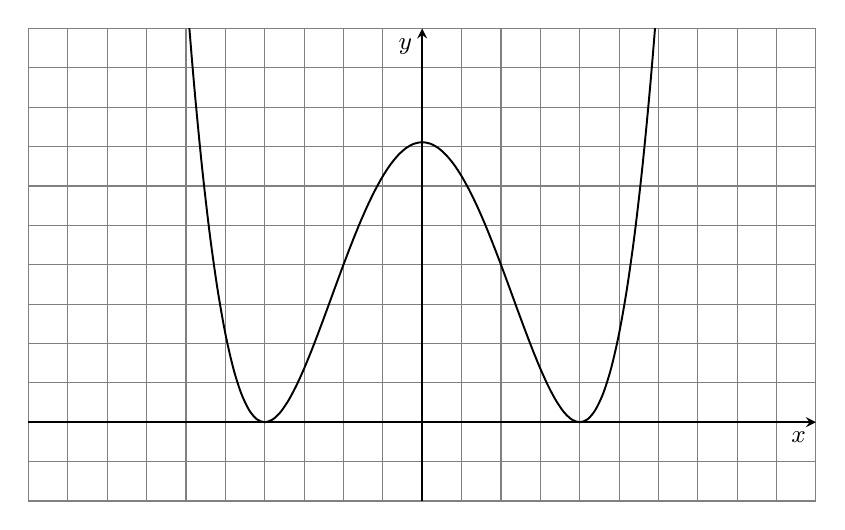
\begin{tikzpicture}[scale=1.000]
        % grid
        \draw[draw=black!50!white] (-5.000, -1.000) grid[step=0.5] (5.000, 5.000);
        % x-axis
        \draw[line width=0.6pt, ->, >=stealth] (-5.000, 0) -- (5.000, 0) node[below left] {\small$x$};
        % y-axis
        \draw[line width=0.6pt, ->, >=stealth] (0, -1.000) -- (0, 5.000) node[below left] {\small$y$};
        % function: f(x)=\num{0.2222222}x^{4}-\num{1.7777778}x^{2}+\num{3.5555556}
        \begin{scope}[line width=0.7pt]
          \clip (-5.000, -1.000) rectangle (5.000, 5.000);
          \draw plot[smooth] coordinates
          {
            ( -5.000,   8.000) ( -4.900,   8.000) ( -4.800,   8.000)
            ( -4.700,   8.000) ( -4.600,   8.000) ( -4.500,   8.000)
            ( -4.400,   8.000) ( -4.300,   8.000) ( -4.200,   8.000)
            ( -4.100,   8.000) ( -4.000,   8.000) ( -3.900,   8.000)
            ( -3.800,   8.000) ( -3.700,   8.000) ( -3.600,   8.000)
            ( -3.500,   8.000) ( -3.400,   8.000) ( -3.300,   8.000)
            ( -3.200,   8.000) ( -3.100,   6.994) ( -3.000,   5.556)
            ( -2.900,   4.322) ( -2.800,   3.277) ( -2.700,   2.405)
            ( -2.600,   1.693) ( -2.500,   1.125) ( -2.400,   0.688)
            ( -2.300,   0.370) ( -2.200,   0.157) ( -2.100,   0.037)
            ( -2.000,   0.000) ( -1.900,   0.034) ( -1.800,   0.128)
            ( -1.700,   0.274) ( -1.600,   0.461) ( -1.500,   0.681)
            ( -1.400,   0.925) ( -1.300,   1.186) ( -1.200,   1.456)
            ( -1.100,   1.730) ( -1.000,   2.000) ( -0.900,   2.261)
            ( -0.800,   2.509) ( -0.700,   2.738) ( -0.600,   2.944)
            ( -0.500,   3.125) ( -0.400,   3.277) ( -0.300,   3.397)
            ( -0.200,   3.485) ( -0.100,   3.538) (  0.000,   3.556)
            (  0.100,   3.538) (  0.200,   3.485) (  0.300,   3.397)
            (  0.400,   3.277) (  0.500,   3.125) (  0.600,   2.944)
            (  0.700,   2.738) (  0.800,   2.509) (  0.900,   2.261)
            (  1.000,   2.000) (  1.100,   1.730) (  1.200,   1.456)
            (  1.300,   1.186) (  1.400,   0.925) (  1.500,   0.681)
            (  1.600,   0.461) (  1.700,   0.274) (  1.800,   0.128)
            (  1.900,   0.034) (  2.000,   0.000) (  2.100,   0.037)
            (  2.200,   0.157) (  2.300,   0.370) (  2.400,   0.688)
            (  2.500,   1.125) (  2.600,   1.693) (  2.700,   2.405)
            (  2.800,   3.277) (  2.900,   4.322) (  3.000,   5.556)
            (  3.100,   6.994) (  3.200,   8.000) (  3.300,   8.000)
            (  3.400,   8.000) (  3.500,   8.000) (  3.600,   8.000)
            (  3.700,   8.000) (  3.800,   8.000) (  3.900,   8.000)
            (  4.000,   8.000) (  4.100,   8.000) (  4.200,   8.000)
            (  4.300,   8.000) (  4.400,   8.000) (  4.500,   8.000)
            (  4.600,   8.000) (  4.700,   8.000) (  4.800,   8.000)
            (  4.900,   8.000) (  5.000,   8.000)
          };
        \end{scope}
      \end{tikzpicture}
      %</OCTAVE>
      %f = [2/9 0 -16/9 0 32/9];
      %mypolyplot(f, -5, 5, -1, 5, 0.1);
    \end{center}
    % </OUTCOME>
  \fi
\end{exercise}
